% Options for packages loaded elsewhere
\PassOptionsToPackage{unicode}{hyperref}
\PassOptionsToPackage{hyphens}{url}
\documentclass[
  man,
  floatsintext]{apa7}
\usepackage{xcolor}
\usepackage{amsmath,amssymb}
\setcounter{secnumdepth}{-\maxdimen} % remove section numbering
\usepackage{iftex}
\ifPDFTeX
  \usepackage[T1]{fontenc}
  \usepackage[utf8]{inputenc}
  \usepackage{textcomp} % provide euro and other symbols
\else % if luatex or xetex
  \usepackage{unicode-math} % this also loads fontspec
  \defaultfontfeatures{Scale=MatchLowercase}
  \defaultfontfeatures[\rmfamily]{Ligatures=TeX,Scale=1}
\fi
\usepackage{lmodern}
\ifPDFTeX\else
  % xetex/luatex font selection
\fi
% Use upquote if available, for straight quotes in verbatim environments
\IfFileExists{upquote.sty}{\usepackage{upquote}}{}
\IfFileExists{microtype.sty}{% use microtype if available
  \usepackage[]{microtype}
  \UseMicrotypeSet[protrusion]{basicmath} % disable protrusion for tt fonts
}{}
\makeatletter
\@ifundefined{KOMAClassName}{% if non-KOMA class
  \IfFileExists{parskip.sty}{%
    \usepackage{parskip}
  }{% else
    \setlength{\parindent}{0pt}
    \setlength{\parskip}{6pt plus 2pt minus 1pt}}
}{% if KOMA class
  \KOMAoptions{parskip=half}}
\makeatother
\usepackage{graphicx}
\makeatletter
\newsavebox\pandoc@box
\newcommand*\pandocbounded[1]{% scales image to fit in text height/width
  \sbox\pandoc@box{#1}%
  \Gscale@div\@tempa{\textheight}{\dimexpr\ht\pandoc@box+\dp\pandoc@box\relax}%
  \Gscale@div\@tempb{\linewidth}{\wd\pandoc@box}%
  \ifdim\@tempb\p@<\@tempa\p@\let\@tempa\@tempb\fi% select the smaller of both
  \ifdim\@tempa\p@<\p@\scalebox{\@tempa}{\usebox\pandoc@box}%
  \else\usebox{\pandoc@box}%
  \fi%
}
% Set default figure placement to htbp
\def\fps@figure{htbp}
\makeatother
% definitions for citeproc citations
\NewDocumentCommand\citeproctext{}{}
\NewDocumentCommand\citeproc{mm}{%
  \begingroup\def\citeproctext{#2}\cite{#1}\endgroup}
\makeatletter
 % allow citations to break across lines
 \let\@cite@ofmt\@firstofone
 % avoid brackets around text for \cite:
 \def\@biblabel#1{}
 \def\@cite#1#2{{#1\if@tempswa , #2\fi}}
\makeatother
\newlength{\cslhangindent}
\setlength{\cslhangindent}{1.5em}
\newlength{\csllabelwidth}
\setlength{\csllabelwidth}{3em}
\newenvironment{CSLReferences}[2] % #1 hanging-indent, #2 entry-spacing
 {\begin{list}{}{%
  \setlength{\itemindent}{0pt}
  \setlength{\leftmargin}{0pt}
  \setlength{\parsep}{0pt}
  % turn on hanging indent if param 1 is 1
  \ifodd #1
   \setlength{\leftmargin}{\cslhangindent}
   \setlength{\itemindent}{-1\cslhangindent}
  \fi
  % set entry spacing
  \setlength{\itemsep}{#2\baselineskip}}}
 {\end{list}}
\usepackage{calc}
\newcommand{\CSLBlock}[1]{\hfill\break\parbox[t]{\linewidth}{\strut\ignorespaces#1\strut}}
\newcommand{\CSLLeftMargin}[1]{\parbox[t]{\csllabelwidth}{\strut#1\strut}}
\newcommand{\CSLRightInline}[1]{\parbox[t]{\linewidth - \csllabelwidth}{\strut#1\strut}}
\newcommand{\CSLIndent}[1]{\hspace{\cslhangindent}#1}
\ifLuaTeX
\usepackage[bidi=basic,shorthands=off]{babel}
\else
\usepackage[bidi=default,shorthands=off]{babel}
\fi
\ifLuaTeX
  \usepackage{selnolig} % disable illegal ligatures
\fi
\setlength{\emergencystretch}{3em} % prevent overfull lines
\providecommand{\tightlist}{%
  \setlength{\itemsep}{0pt}\setlength{\parskip}{0pt}}
% preamble.tex 

\usepackage{csquotes}
\usepackage{amsmath}
\usepackage{amssymb}
\usepackage{graphicx}
\usepackage{subcaption}
\usepackage{caption}
\usepackage{geometry}
\usepackage{float}
\usepackage{rotating}


\captionsetup{justification=raggedright,singlelinecheck=false}

\shorttitle{SEMI-COMPLETE BY DESIGN}
\affiliation{$^{1}$Goethe University Frankfurt\\ $^{2}$Max Planck Institute for Human Development{,} Berlin{,} Germany\\ $^{3}$MSB Medical School Berlin{,} Berlin{,} Germany\\ $^{4}$Max Planck UCL Centre for Computational Psychiatry and Ageing Research{,} Berlin{,} Germany}
\usepackage{placeins}
\setlength{\textfloatsep}{6pt}
\setlength{\floatsep}{6pt}
\setlength{\intextsep}{6pt}
\raggedbottom
\usepackage{bookmark}
\IfFileExists{xurl.sty}{\usepackage{xurl}}{} % add URL line breaks if available
\urlstyle{same}
\hypersetup{
  pdftitle={SEMi-Complete by Design: A Monte Carlo simulation to assess Measurement Invariance in Moderated Nonlinear Factor Analysis and SEM-Trees},
  pdfauthor={Leonie Hagitte\^{}\{1,2,3\}, Andreas M. Brandmaier\^{}\{2,3,4\}},
  pdflang={american},
  hidelinks,
  pdfcreator={LaTeX via pandoc}}

\title{SEMi-Complete by Design: A Monte Carlo simulation to assess
Measurement Invariance in Moderated Nonlinear Factor Analysis and
SEM-Trees}
\author{Leonie Hagitte\(^{1,2,3}\), Andreas M. Brandmaier\(^{2,3,4}\)}
\date{2025-12-10}

\begin{document}
\maketitle

\section{General Information}\label{general-information}

\subsection{What is the title of the
project?}\label{what-is-the-title-of-the-project}

SEMi-Complete by Design: A Monte Carlo simulation to assess Measurement
Invariance in Moderated Nonlinear Factor Analysis and SEM-Trees.

\subsection{Who are the current and future project
contributors?}\label{who-are-the-current-and-future-project-contributors}

Leonie Hagitte, Andreas M. Brandmaier

\subsection{Provide a description of the
project.}\label{provide-a-description-of-the-project.}

Ensuring the validity of psychological assessments is crucial, yet
differential item functioning (DIF) can threaten measurement invariance
(MI) when test items function differently across groups (Bauer et al.
2020). Recent calls for improved DIF detection methods emphasize the
need for more advanced statistical approaches (Lee et al. 2024).
Moderated nonlinear factor analysis (MNLFA) is a recent approach for
assessing MI via parameter moderation within a single-group confirmatory
factor analysis framework (Bauer 2017). MLNFA evaluates MI across
multiple continuous and categorical covariates, and accounts for
heteroskedasticity by modeling factor and residual variances as
functions of these covariates. While MNLFA offers continuous moderation
of several parameters of SEMs (e.g.: factor loadings, covariances etc.),
it requires a priori specification of covariates and their functional
relationships, which are usually assumed to be linear (Bauer 2017; Kolbe
et al. 2024). In contrast, structural equation modeling (SEM) trees and
forests are data-driven, non-parametric methods that use recursive
partitioning to identify latent subgroups in which model parameters
differ, without assuming specific functional forms or predefined
covariate effects. These approaches allow for nonlinear moderation of
factor loadings and can reveal complex interaction effects, enabling the
exploratory detection of DIF (Brandmaier et al. 2016, 2013). In this
study, we conducted a Monte Carlo simulation to compare the performance
of MNLFA and SEM trees and forests in detecting DIF and assessing MI
under varying conditions. Specifically, we evaluate their effectiveness
in identifying non-invariance and detecting relevant covariates. Our
findings will inform best practices for selecting statistical techniques
to test MI in psychological assessment.

\subsection{Did any of the contributors already conduct related
simulation studies on this specific
question?}\label{did-any-of-the-contributors-already-conduct-related-simulation-studies-on-this-specific-question}

Neither of the authors has conducted simulation studies that are of
immediate relevance to the current project before. However, Andreas
Brandmaier was involved in conducting simulation studies on SEM trees/
SEM forests as well as SEM modeling in general (e.g., Buchberger et al.
2024; Díaz et al. 2025; Arnold et al. 2021).

\section{Aims}\label{aims}

\subsection{What is the aim of the simulation
study?}\label{what-is-the-aim-of-the-simulation-study}

The aim of this simulation study is to evaluate different methods
(i.e.~MNLFA and SEM trees/ SEM forests) regarding their accuracy, power,
and false-positive rate in detecting MI across different factor models
(ADEMP category `hypothesis testing').

\section{Data-Generating Mechanism}\label{data-generating-mechanism}

\subsection{How will the parameters for the data-generating mechanism
(DGM) be
specified?}\label{how-will-the-parameters-for-the-data-generating-mechanism-dgm-be-specified}

The data will be generated parametrically. Different population
structural equation models (SEM) with latent variables and continuous
indicators will be simulated in two different simulation studies:

\subsection{Study 1}\label{study-1}

\textbf{Single-Factor Model with Moderated Parameters}

We specify a confirmatory factor analysis model (model 1) with a single
latent factor \(\eta\) and four observed indicators
\(\mathbf{x} = (x_1, \dots, x_4)^\top\). The influence of continuous
moderator variables is introduced into selected parameters via
predefined transformation functions applied to underlying raw moderator
variables.\\
The population model is:

\[
\mathbf{x} = \boldsymbol{\nu}(Z) + \boldsymbol{\Lambda}_x(Z)\,\eta + \boldsymbol{\varepsilon},
\qquad
\boldsymbol{\varepsilon} \sim \mathcal{N}(\mathbf{0}, \boldsymbol{\Theta}_\varepsilon).
\]

where

\begin{itemize}
\tightlist
\item
  \(\boldsymbol{\nu}(Z)\) is the vector of intercepts,
\item
  \(\boldsymbol{\Lambda}_x(Z)\) is the \(4 \times 1\) factor loading
  matrix,
\item
  \(\boldsymbol{\varepsilon} \sim \mathcal{N}\!\left(\mathbf{0}, \boldsymbol{\Theta}_\varepsilon\right)\)
  is the residual vector,
\item
  \(\eta \sim \mathcal{N}(0,1)\) is the latent factor,
\item
  \(Z = h(M)\) denotes the effective moderator entering the model
  equations, obtained by transforming one or more raw continuous
  moderator variables.
\end{itemize}

\subsubsection{Moderator Transformation}\label{moderator-transformation}

Let \(M \sim \mathcal{U}(-1,1)\) denote a bounded uniformly distributed
continuous covariate.

The effective moderator is defined as \[
Z = h(M),
\]

where \(h(\cdot)\) is chosen from the following deterministic
transformation functions. Each transformation type is treated as a
distinct condition in the simulation design:

\begin{enumerate}
\def\labelenumi{\arabic{enumi}.}
\item
  \textbf{Linear:} \[
  h(M) = M
  \] In this case, the effective moderator is bounded to the interval
  \((-1,1)\) and rotation symmetric around zero.
\item
  \textbf{Sigmoid:} \[
  h(M) = a + \frac{b-a}{1 + \exp\!\bigl(-k(M-c)\bigr)},
  \qquad a=-1,\; b=1,\; c=0,\; k=10.
  \] This transformation maps the input to the open interval \((-1, 1)\)
  and yields a bounded moderator, rotation symmetric around zero,
  exhibiting diminishing sensitivity at extreme values.
\item
  \textbf{Quadratic:} \[
  h(M) = 2M^2 - 1
  \] This transformation captures symmetric nonlinear moderation as a
  function of distance from the center while remaining bounded in
  \((-1,1)\).
\item
  \textbf{Noise:} \[
  h(M) = 0
  \] In this condition, the effective moderator is constant and
  therefore has no effect on any model parameter. Although this
  condition is termed ``noise'' in the simulation code, it represents
  the absence of systematic moderation rather than a randomly varying
  noise effect.
\end{enumerate}

The absence of moderation is represented by the noise-moderator
condition \((Z=0)\), not by setting \(\delta=0\); moderation
coefficients are held fixed across conditions. All parameter-level
moderation effects are specified as linear functions of the effective
moderator \(Z\). Nonlinearity in moderation arises exclusively through
the transformation \(Z = h(M)\), not through nonlinear parameter
functions. The transformation \(h(M)\) is part of the DGM in every
moderation condition.

\begin{figure}

{\centering 
\includegraphics[width=0.9\linewidth]{newprereg_files/figure-latex/fig-moderation-functions-1} 

}

\caption{Note. The dashed horizontal line indicates the null moderation case (noise: $\delta h(M) = 0$ for all $M$). The moderation strength for the latent covariance shares the same $\delta$ values as $\delta_{\lambda} \in \{0.2, 0.3\}$.}\label{fig:fig-moderation-functions}
\end{figure}

\subsubsection{Factor Loadings}\label{factor-loadings}

The baseline factor loadings were fixed to a discrete value of
\(\lambda_{xi} = 0.7\).\\
Variation in factor loadings across simulation conditions arises
exclusively through continuous moderator effects specified in the
population model.

\subsubsection{Moderated items}\label{moderated-items}

At the population level, the baseline (unmoderated) measurement model is
specified with a single latent factor and four indicators. The factor
loading matrix is constructed such that all four indicators share a
common loading value \(\lambda\):

\[
\boldsymbol{\Lambda}_x =
\begin{bmatrix}
\lambda_1 \\
\lambda_2 \\
\lambda_3 \\
\lambda_4
\end{bmatrix}
\]

The latent factor variance is fixed at a prespecified constant value
\(\psi_{\eta}= 1\) and is held constant across all simulation
conditions.

For each condition involving moderation, the loading of item \(i\) is
defined as a deterministic function of the moderator \(Z\):

\[
\lambda_{xi}(Z) = \lambda_{xi} + \delta_{\lambda} Z,
\quad Z \in [-1, 1].
\]

The parameter \(\delta_{\lambda}\) represents the strength of the
moderation effect and is specified using a discrete set of admissible
values chosen to ensure that the moderated loading remains within a
psychometrically plausible interval:

\[
\lambda_{xi}(Z) \in [0.3,\, 1.0].
\]

Given the fixed baseline loading \(\lambda_{xi}=0.7\), this constraint
yields an admissible range \[
\delta_{\lambda} \in [-0.4,\, 0.3].
\]

\(\delta_{\lambda}\) is evaluated at the following discrete levels:

\[
\delta_\lambda\in\{0.20,0.30\}.
\]

For moderator transformations beyond the linear case (quadratic or
sigmoid), the functional form of \(\lambda_{xi}(Z)\) is adapted
accordingly, and the same discrete set of admissible moderation
strengths is applied. This yields crossed combinations of (i) moderator
transformation, (ii) moderated parameter type, (iii) number of moderated
items, and (iv) moderation strength.

\subsubsection{Factor loading matrix}\label{factor-loading-matrix}

\[
\boldsymbol{\Lambda}_x(Z) =
\begin{bmatrix}
\lambda_1(Z) \\
\lambda_2(Z) \\
\lambda_3(Z)\\
\lambda_4(Z)
\end{bmatrix}
\]

Loading moderation is manipulated via the pattern of moderated items and
the magnitude of the moderation effect. For each indicator \(i\), the
loading is modeled as

\[
\lambda_i(Z) = \lambda_i + \delta_{\lambda} Z,
\]

where \(\lambda_i\) denotes the baseline loading and
\(\delta_{\lambda}\) controls the strength and direction of loading
moderation.

\textbf{No loading moderation:}\\
\[
\delta_{\lambda}=0 \quad \text{for all } i=1,\dots,4.
\]

\textbf{Partial loading moderation:}\\
Only the loadings of items 1 and 2 vary with \(Z\):

\[
\delta_{\lambda} \in \{0.20,0.30\}
\quad \text{for } i \in \{1,2\},
\qquad
\delta_{\lambda}=0
\quad \text{for } i \in \{3,4\}.
\]

\textbf{Full loading moderation:}\\
All four loadings vary with \(Z\):

\[
\delta_{\lambda} \in \{-0.3,-0.2,0.2,0.3\}
\quad \text{for } i=1,\dots,4.
\]

\subsubsection{Residual variances}\label{residual-variances}

Residual variances were chosen such that all four indicators had a
reliability of

\[
\rho = .75.
\]

Given the fixed latent variance

\[
\psi_\eta = 1
\]

and baseline loading

\[
\lambda_i = 0.70,
\]

baseline residual variances were computed as

\[
\theta_i =
\frac{\lambda_i^2\psi_\eta(1-\rho)}
{\rho}.
\]

Residual variances were held constant across all simulation conditions.
Consequently, when factor loadings were moderated, indicator reliability
varied as a function of the moderator.

\subsubsection{Intercepts}\label{intercepts}

Intercept moderation is manipulated via the pattern of moderated items
and the magnitude of the moderation effect. For each indicator \(i\),
the intercept is modeled as

\[
\nu_i(Z) = \nu_i + \delta_{\nu} Z,
\]

where \(\nu_i\) denotes the baseline intercept and \(\delta_{\nu}\)
controls the strength and direction of intercept moderation.

\textbf{No intercept moderation:}\\
\[
\delta_{\nu}=0 \quad \text{for all } i=1,\dots,4.
\]

\textbf{Partial intercept moderation:}\\
Only the intercepts of items 1 and 2 vary with \(Z\):

\[
\delta_{\nu} \in \{0.5,1.0\}
\quad \text{for } i \in \{1,2\},
\qquad
\delta_{\nu}=0
\quad \text{for } i \in \{3,4\}.
\]

\textbf{Full intercept moderation:}\\
All four intercepts vary with \(Z\):

\[
\delta_{\nu} \in \{0.5,1.0\}
\quad \text{for } i=1,\dots,4.
\]

Baseline intercepts are set to 1 across simulation conditions.

\newpage

\subsubsection{Population model
overview}\label{population-model-overview}

The population models are generated by combining the loading- and
intercept-moderation specifications above.

\begin{table}[!htbp]
\centering
\caption{Population models defined by loading and intercept moderation specifications.}
\label{tab:population-models}
\begin{tabular}{llll}
\toprule
Model & Loading moderation & Intercept moderation & Active moderator structure \\
\midrule
0    & none & none & none \\
1.1  & full & none & $Z_1 = h(M_1)$ \\
1.11 & none & full & $Z_1 = h(M_1)$ \\
1.12 & full & full & $Z_1 = h(M_1)$ \\
1.2  & partial, items 1--2 & none & $Z_1 = h(M_1)$ \\
1.21 & none & partial, items 1--2 & $Z_1 = h(M_1)$ \\
1.22 & partial, items 1--2 & partial, items 1--2 & $Z_1 = h(M_1)$ \\
1.3  & full & none & $Z_1 = h(M_1)$, $Z_2 = h(M_2)$, $Z_1Z_2$ \\
1.32 & full & full & $Z_1 = h(M_1)$ (loadings), $Z_2 = h(M_2)$ (intercepts) \\
\bottomrule
\end{tabular}
\end{table}

For Model 1.3, the loading equation is: \[
\lambda_i(Z_1,Z_2) =
\lambda_i
+ \delta_{\lambda }Z_1
+ \delta_{\lambda }Z_2
+ \delta_{\lambda }^{2}Z_1Z_2
\]

Specifically, the moderation coefficients are defined as

\[
\delta_{\lambda 1}
=
\delta_{\lambda 2}
=
\delta_{\lambda},
\qquad
\delta_{\lambda 12}
=
\delta_{\lambda}^{2}.
\]

For Model 1.32, loading and intercept moderation depend on separate
moderators:

\[
\lambda_i(Z_1)
=
\lambda_i
+
\delta_{\lambda}Z_1,
\]

and

\[
\nu_i(Z_2)
=
\nu_i
+
\delta_{\nu}Z_2.
\]

\subsubsection{Latent distribution}\label{latent-distribution}

The latent factor is assumed to follow a standard normal distribution,

\[
\eta \sim \mathcal{N}(0,1),
\]

so that the latent mean is fixed at 0 and the latent variance is fixed
at 1 across all simulation conditions.

\pagebreak

\subsubsection{Analytical Model Study 1}\label{analytical-model-study-1}

\vspace*{1em}

\begin{figure}

{\centering 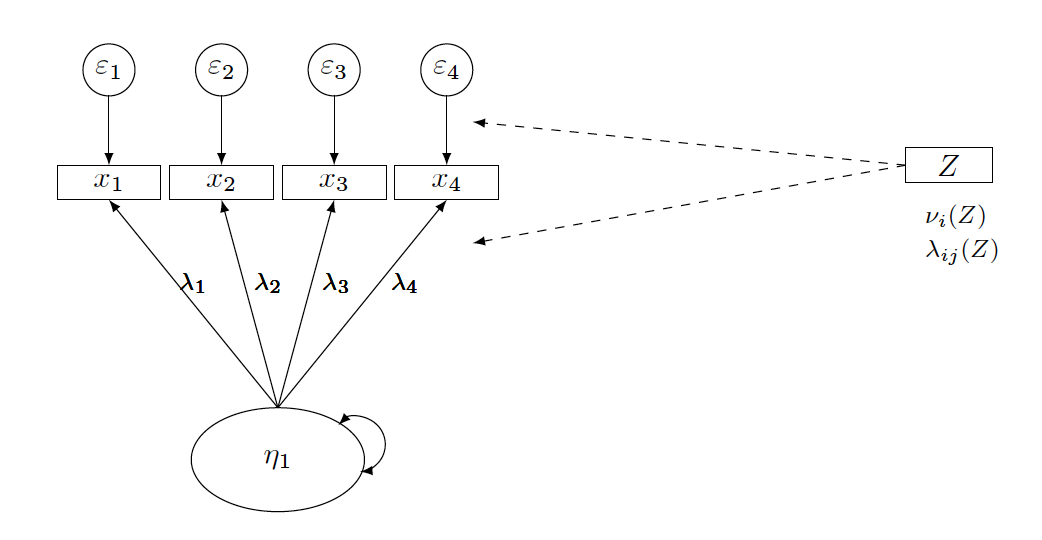
\includegraphics[width=0.7\linewidth]{tikz_model1} 

}

\caption{Note. Conceptual depiction of used Analytical Models.}\label{fig:fig-model2}
\end{figure}

The analytical model will contain one latent factor \(\eta_1\), with
four manifest indicators \({x_1,..., x_4}\), their factor loadings
\({\lambda_1,..., \lambda_4}\) and their respective residuals
\({\epsilon_1,..., \epsilon_4}\) (See Figure 2). Residual variances are
freely estimated, and residual covariances are fixed to zero.\\
For MNLFA, moderation of selected factor loadings and intercepts is
modeled parametrically. Two analytical MNLFA specifications are
considered. In the linear specification, measurement parameters are
modeled as linear functions of the raw moderator \(M\). In the quadratic
specification, the moderator entering the MNLFA is transformed as
\(2M^2-1\). In the main study, two MNLFA specifications will be
evaluated: one assuming linear moderation in the observed moderator(s),
and one assuming quadratic moderation. Therefore, MNLFA is correctly
specified only when the analytical functional form matches the DGM
transformation \(h(M)\), and is otherwise intentionally misspecified.
For population models involving a single moderator, MNLFA includes the
corresponding observed moderator as the predictor of measurement
parameters. For population models involving a single moderator, MNLFA
includes the corresponding observed moderator as the predictor of
measurement parameters. For the interaction population model (Model
1.3), the analytical model additionally includes the interaction term
\(M_1 \times M_2\). For Model 1.32, separate observed moderators
(\(M_1\) and \(M_2\)) are included for loading and intercept moderation,
respectively.

\subsection{What will be the different factors of the data-generating
mechanism?}\label{what-will-be-the-different-factors-of-the-data-generating-mechanism}

The simulation design includes several manipulated factors governing the
data-generating mechanism (DGM). These factors are systematically
crossed to generate the simulation conditions. The population models are
summarized in Table 1.

\subsubsection{Core DGM Factors}\label{core-dgm-factors}

The following factors are systematically varied in the study using a
grid search design:

\paragraph{Functional form of
moderation}\label{functional-form-of-moderation}

The functional form relating the raw moderator to the effective
moderator is varied across the following deterministic transformations:

\begin{enumerate}
\def\labelenumi{\arabic{enumi}.}
\tightlist
\item
  Linear\\
\item
  Quadratic\\
\item
  Sigmoid\\
\item
  Noise/null transformation, \(h(M)=0\)
\end{enumerate}

\paragraph{Strength of moderation}\label{strength-of-moderation}

In each case where parameters are subjected to moderation, the strength
of the moderation \(\delta\) is varied:

\(\delta_{\lambda}\) is evaluated at the following discrete levels:

\[
\delta_{\lambda} \in \{0.2,\,0.3\}.
\] whereas intercept moderation is evaluated using

\[
\delta_{\nu} \in \{0.5,\,1.0\}.
\] \#\#\#\# Population Model

Nine population models are considered, differing in the presence and
pattern of loading moderation, intercept moderation, and moderator
structure (Table 1).

\paragraph{Model misspecification of moderator
form}\label{model-misspecification-of-moderator-form}

The DGM always defines moderation through the transformed moderator
\(Z=h(M)\). Linear and quadratic MNLFA impose corresponding parametric
moderation functions. Consequently, each MNLFA specification is
correctly specified only when its assumed functional form matches the
population model and is intentionally misspecified otherwise. SEM trees
do not assume a parametric moderator function but instead identify MNI
through recursive partitioning of the observed moderator variables.

\paragraph{Limitations of the Core
DGM}\label{limitations-of-the-core-dgm}

The simulation assumes that the moderators are measured without error.
Consequently, the results reflect an idealized setting in which
moderation effects are perfectly observed. Introducing measurement error
in the moderators would likely reduce statistical power and estimation
accuracy but is beyond the scope of the present study.

\subsubsection{Simulation Design
Factors}\label{simulation-design-factors}

The factorial simulation design crosses the following manipulated
factors:

\begin{itemize}
\tightlist
\item
  Population model (9 levels; Table\textasciitilde1)
\item
  Moderator transformation (linear, quadratic, sigmoid, noise/null)
\item
  Loading moderation magnitude (\(\delta_\lambda\in\{0.20,0.30\}\))
\item
  Intercept moderation magnitude (\(\delta_\nu\in\{0.50,1.00\}\))
\item
  Sample size (\(N\in\{250,500,1000\}\))
\item
  Analysis method (linear MNLFA, quadratic MNLFA, SEM Trees)
\end{itemize}

\subsubsection{If there is more than one factor: How will the factor
levels be combined and how many simulation conditions will this
create?}\label{if-there-is-more-than-one-factor-how-will-the-factor-levels-be-combined-and-how-many-simulation-conditions-will-this-create}

We employ a full grid search, in which parameter values are sampled from
pre-specified discrete values. A total of 6,000 simulation replications
should ideally be conducted. This number was chosen to ensure that the
confidence intervals for key estimated proportions (e.g., power or Type
I error rates near a binomial success probability of \(p = 0.8\) achieve
an approximate width of \(\pm 1\%\). This is based on the calculation:

\[
\text{SE} = 2 \times \sqrt{\frac{p(1-p)}{6000}},
\]

which yields a standard error consistent with the desired precision for
evaluating simulation outcomes within this study.

The implemented simulation employed a fully crossed factorial design.
Crossing the nine population models, four moderator transformations, two
loading-moderation magnitudes, two intercept-moderation magnitudes, and
four sample sizes yielded 576 unique data-generating design cells. Each
generated dataset was analyzed using three analytical methods (linear
MNLFA, quadratic MNLFA, and SEM Trees), resulting in 1,728
method-specific analysis conditions. To ensure computational
feasibility, each condition is replicated 100 times. In addition, one
SEM Tree sensitivity condition evaluates the influence of ten irrelevant
moderator variables.

\subsection{Estimands and Targets}\label{estimands-and-targets}

\subsubsection{What will be the estimands and/or targets of the
simulation
study?}\label{what-will-be-the-estimands-andor-targets-of-the-simulation-study}

The primary estimands in this simulation study pertain to the detection
and accurate estimation of MNI due to moderation effects on measurement
parameters. Specifically, we assess whether the estimation methods
compared can correctly identify the presence or absence of moderation in
factor loadings and intercepts, reflecting the true data-generating
structure. Consequently, key simulation outcomes include Type I error
rates and statistical power associated with detecting such moderation
effects.

\subsection{Methods}\label{methods}

\subsubsection{How many and which methods will be included and which
quantities will be
extracted?}\label{how-many-and-which-methods-will-be-included-and-which-quantities-will-be-extracted}

We will compare the following methods:

\begin{enumerate}
\def\labelenumi{\arabic{enumi})}
\item
  \textbf{Moderated Nonlinear Factor Analysis:} MNLFA was initially
  introduced by Bauer and Hussong (2009) within the framework of
  integrative data analysis and was subsequently extended into a general
  approach for assessing measurement invariance and moderation (Bauer
  2017). The fundamental principle of MNLFA is the parameterization of
  both measurement and structural model parameters as functions of one
  or more moderator variables. MNLFA accommodates both frequentist
  estimation methods, such as maximum likelihood (ML), and Bayesian
  techniques, including Markov Chain Monte Carlo (MCMC), thereby
  offering methodological flexibility aligned with specific analytical
  objectives (Münch and Koch 2024).
\item
  \textbf{SEM Trees:} Structural equation modeling (SEM) trees were
  originally introduced by Brandmaier et al. (2013) as a way to
  systematically search for important covariates and their interactions
  in data, creating homogeneous subgroups. The method was refined later
  on by Brandmaier et al. (2016) and Arnold et al. (2021). SEM trees and
  forests are data-driven, non-parametric methods that build upon the
  decision tree paradigm, thus using recursive partitioning to identify
  latent subgroups in which model parameters differ, without assuming
  specific functional forms or predefined covariate effects. These
  approaches allow for nonlinear moderation of factor loadings and can
  reveal complex interaction effects, enabling the exploratory detection
  of DIF.
\end{enumerate}

For the parametric MNLFA, we will extract estimated moderated parameters
(e.g., factor loadings, intercepts), their associated standard errors,
and two-sided \(p\)-values for testing the null hypothesis of no
moderation effect. Additionally, model fit indices such as AIC and the
LRT-statistics will be recorded.

For the parameter estimates and fit indices, we will summarize their
distributions across simulation replications by reporting key quantiles
(2.5th, 50th, and 97.5th percentiles). The null hypothesis will be
rejected if the associated \(p\)-value is less than the conventional
significance level of 0.05.

In contrast, non-parametric tree-based approaches do not yield direct
parameter estimates with standard errors. We use score-based
SEM-trees(Arnold et al. 2021). Their detection of MI/ non-invariance is
operationalized via the presence of at least one split in the correct
condition at the correct respective level of focus parameters. Those
splits, introducing a subgroup, will be evaluated at the significance
level: 0.05. Additionally, a Bonferroni correction to account for
multiple comparisons at each node. The trees will be allowed to split on
the focus parameters relevant for the invariance testing (the means of
the intercepts, factor loadings and the latent covariance in study 2).
Candidate subgroup structures are assessed by testing whether they
produce statistically significant differences in the specified model
parameters across groups. Differences in factor variances between
subgroups are permitted in the model, but they are not used as criteria
for selecting or evaluating covariates. Furthermore, pre-pruning will be
applied, limiting the maximum depth of the tree to 3 and \texttt{min.N}
is set to 50. Because the MNLFA also considers directly the form of the
moderation, which the SEM trees do not, we further want to use SEM
forests for generating partial dependence plots to get an approximation
of the functional form of the moderating variables.\\
With this distinction we aim to ensure that each method is evaluated
according to its own inferential framework, while maintaining
comparability in terms of its ability to detect MI reliably.

\subsection{Performance Measures}\label{performance-measures}

\subsubsection{Which performance measures will be
used?}\label{which-performance-measures-will-be-used}

For both the MNLFA approaches and SEM Trees, the primary performance
measures concern the detection of MNI.

\textbf{Type I Error Rate and Power:} The rejection rate of the null
hypothesis at significance level \(\alpha = 0.05\), calculated as \[
\widehat{\text{RRate}} = \frac{1}{n_{\text{sim}}} \sum_{i=1}^{n_{\text{sim}}} \mathbf{1}(p_i \leq 0.05),
\]

where \(\mathbf{1}(\cdot)\) is the indicator function.

Performance measures calculated for multiple moderated parameters (e.g.,
factor loadings or intercepts) will be summarized separately for loading
and intercept moderation and, where appropriate, aggregated across
parameters.

For the MNLFA approaches, parameter recovery will additionally be
evaluated by comparing the estimated moderation parameters with their
corresponding population values. The following classical Monte Carlo
performance measures will be used:

\textbf{Bias:} The average difference between the estimated parameter
\(\hat{\theta}\) and the true parameter \(\theta\), defined as \[
\widehat{\text{Bias}} = \frac{1}{n_{\text{sim}}} \sum_{i=1}^{n_{\text{sim}}} \hat{\theta}_i - \theta,
\] where \(n_{\text{sim}}\) is the number of simulation replications.

\textbf{Absolute Bias:} \[
\widehat{\text{AbsBias}} = \frac{1}{n_{\text{sim}}} \sum_{i=1}^{n_{\text{sim}}} \left| \hat{\theta}_i - \theta \right|.
\]

\textbf{Relative Bias:} (expressed as a proportion of the true
parameter) \[
\widehat{\text{RelBias}} = \frac{\widehat{\text{Bias}}}{|\theta|} \quad \text{for } \theta \neq 0.
\]

\textbf{Root Mean Squared Error (RMSE):} \[
\widehat{\text{RMSE}} = \sqrt{ \frac{1}{n_{\text{sim}}} \sum_{i=1}^{n_{\text{sim}}} (\hat{\theta}_i - \theta)^2}.
\]

\textbf{Coverage Probability:} The proportion of confidence intervals
that contain the true parameter \(\theta\).

\subsubsection{How will Monte Carlo uncertainty of the estimated
performance measures be calculated and
reported?}\label{how-will-monte-carlo-uncertainty-of-the-estimated-performance-measures-be-calculated-and-reported}

Monte Carlo uncertainty will be quantified using Monte Carlo standard
errors (MCSEs) for the estimated performance measures.

The \textbf{Rejection Rate} refers to the proportion of simulated
datasets in which a null hypothesis is rejected, commonly used to
estimate empirical Type I error rates or statistical power.

The \textbf{MCSE for the Rejection Rate} is calculated assuming a
binomial distribution of rejections across \(n_{\text{sim}}\) simulation
replications, which reflects the standard error of a proportion
estimator:

\[
\text{MCSE}_{\widehat{\text{RRate}}} = \sqrt{\frac{\widehat{\text{RRate}} (1 - \widehat{\text{RRate}})}{n_{\text{sim}}}},
\]

For \textbf{Bias}, MCSE is calculated based on the sample variance of
the specific parameter estimates across simulation replications:

\[
\text{MCSE}_{\widehat{\text{Bias}}} = \frac{S_{\hat{\theta}}}{\sqrt{n_{\text{sim}}}},
\]

where \[
S_{\hat{\theta}} = \sqrt{\sum_{i=1}^{n_{\text{sim}}}{ \{\hat{\theta}_i - (\sum_{i=1}^{n_{\text{sim}}}\hat{\theta}_i/n_{\text{sim}})\}^2}/(n_{\text{sim}} - 1)}
\] is the sample standard deviation of the effect estimates.

Siepe et al. (2024) ,Morris et al. (2019) and Whitehead (1993)

\subsection{How many simulation repetitions will be used for each
condition?}\label{how-many-simulation-repetitions-will-be-used-for-each-condition}

The number of simulation repetitions and how we derived them is
described above under ``If there is more than one factor: How will the
factor levels be combined and how many simulation conditions will this
create?''.

\subsection{How will missing values due to non-convergence or other
reasons be
handled?}\label{how-will-missing-values-due-to-non-convergence-or-other-reasons-be-handled}

Non-convergence or other missing values may occur during model
estimation. We plan to:

\begin{itemize}
\tightlist
\item
  Exclude only the specific simulation replicates that fail to converge
  for a given method while retaining data from other methods within the
  same replication.
\item
  Report the proportion of non-converged cases per method and condition.
\item
  If the proportion of non-convergence exceeds a pre-specified threshold
  (e.g., 5\%), we will flag the corresponding simulation condition and
  interpret results with caution.
\end{itemize}

No imputation of missing estimates will be performed.

\subsection{How do you plan on interpreting the performance
measures?}\label{how-do-you-plan-on-interpreting-the-performance-measures}

The performance measures will be interpreted in terms of Type I error
rates and statistical power. Type I error is defined as the proportion
of replications in which a method incorrectly detects measurement
noninvariance when none is present. Statistical power is defined as the
proportion of replications in which a method correctly detects
measurement noninvariance when it is truly present.

Results will be evaluated both overall and conditional on design
factors. Particular attention will be paid to whether Type I error rates
are controlled at nominal levels and how power varies as a function of
effect size and data-generating conditions. Comparisons between methods
will focus on their relative sensitivity to different forms of
noninvariance (metric vs scalar) and robustness across conditions.

\section{Other}\label{other}

\subsection{Which statistical software/packages do you plan to
use?}\label{which-statistical-softwarepackages-do-you-plan-to-use}

All simulations and analyses will be conducted in R (R Core Team 2025).
The MNLFA-style models will be implemented directly in
\texttt{OpenMx}(Boker et al. 2026), using raw-data maximum likelihood
estimation and definition-variable-style moderation through OpenMx
algebra objects. SEM tree analyses will be performed with the
\texttt{semtree} (Brandmaier et al. 2026) package using OpenMx RAM
models. Simulation design construction, data handling, aggregation, and
visualization will rely on \texttt{dplyr}(Wickham et al. 2026),
\texttt{tidyr} (Wickham et al. 2025), \texttt{tibble} (Müller and
Wickham 2026), \texttt{purrr} (Wickham and Henry 2026), \texttt{furrr}
(Vaughan and Dancho 2022), \texttt{future} (Bengtsson 2021),
\texttt{parallel} (R Core Team 2025), and \texttt{ggplot2} (Wickham
2016).

\subsection{Which computational environment do you plan to
use?}\label{which-computational-environment-do-you-plan-to-use}

The simulation study will be conducted in R (R Core Team 2025).

\subsection{Which other steps will you undertake to make simulation
results
reproducible?}\label{which-other-steps-will-you-undertake-to-make-simulation-results-reproducible}

We are planning to make the code of this project publicly available.
Software and packages will be documented via \texttt{renv}(Ushey and
Wickham 2026) and Docker. Furthermore, we are planning to use the
\texttt{repro} package, as well as the \texttt{reproducibleRchunks}
package for better reproducibility.

\pagebreak

\subsection*{References}\label{references}
\addcontentsline{toc}{subsection}{References}

\protect\phantomsection\label{refs}
\begin{CSLReferences}{1}{1}
\bibitem[\citeproctext]{ref-Arnold2021}
Arnold, M., M. C. Voelkle, and A. M. Brandmaier. 2021. {``Score-Guided
Structural Equation Model Trees.''} \emph{Frontiers in Psychology} 11:
3913. \url{https://doi.org/10.3389/fpsyg.2020.564403}.

\bibitem[\citeproctext]{ref-Bauer2017}
Bauer, D. J. 2017. {``A More General Model for Testing Measurement
Invariance and Differential Item Functioning.''} \emph{Psychological
Methods} 22 (3): 507--26. \url{https://doi.org/10.1037/met0000077}.

\bibitem[\citeproctext]{ref-Bauer2020}
Bauer, D. J., W. C. M. Belzak, and V. T. Cole. 2020. {``Simplifying the
Assessment of Measurement Invariance over Multiple Background Variables:
Using Regularized Moderated Nonlinear Factor Analysis to Detect
Differential Item Functioning.''} \emph{Structural Equation Modeling: A
Multidisciplinary Journal} 27 (1): 43--55.
\url{https://doi.org/10.1080/10705511.2019.1642754}.

\bibitem[\citeproctext]{ref-Bauer2009}
Bauer, D. J., and A. M. Hussong. 2009. {``Psychometric Approaches for
Developing Commensurate Measures Across Independent Studies: Traditional
and New Models.''} \emph{Psychological Methods} 14 (2): 101--25.
\url{https://doi.org/10.1037/a0015583}.

\bibitem[\citeproctext]{ref-future2021}
Bengtsson, Henrik. 2021. {``A Unifying Framework for Parallel and
Distributed Processing in r Using Futures.''} \emph{The R Journal} 13
(2): 208--27. \url{https://doi.org/10.32614/RJ-2021-048}.

\bibitem[\citeproctext]{ref-Boker2026}
Boker, Steven M., Michael C. Neale, Hermine H. Maes, et al. 2026.
\emph{OpenMx: Extended Structural Equation Modelling}.
\url{https://doi.org/10.32614/CRAN.package.OpenMx}.

\bibitem[\citeproctext]{ref-Brandmaier2013}
Brandmaier, A. M., T. von Oertzen, J. J. McArdle, and U. Lindenberger.
2013. {``Structural Equation Model Trees.''} \emph{Psychological
Methods} 18 (1): 71--86. \url{https://doi.org/10.1037/a0030001}.

\bibitem[\citeproctext]{ref-Brandmaier2016}
Brandmaier, A. M., J. J. Prindle, J. J. McArdle, and U. Lindenberger.
2016. {``Theory-Guided Exploration with Structural Equation Model
Forests.''} \emph{Psychological Methods} 21 (4): 566--82.
\url{https://doi.org/10.1037/met0000090}.

\bibitem[\citeproctext]{ref-semtree2026}
Brandmaier, A. M., John J. Prindle, Manuel Arnold, and Caspar J. Van
Lissa. 2026. \emph{Semtree: Recursive Partitioning for Structural
Equation Models}. \url{https://github.com/brandmaier/semtree}.

\bibitem[\citeproctext]{ref-Buchberger2024}
Buchberger, E. S., C. T. Ngo, A. Peikert, A. M. Brandmaier, and M.
Werkle-Bergner. 2024. {``Estimating Statistical Power for Structural
Equation Models in Developmental Cognitive Science: A Tutorial in r.''}
\emph{Behavior Research Methods} 56 (7): 6862--79.
\url{https://doi.org/10.3758/s13428-024-02396-2}.

\bibitem[\citeproctext]{ref-SilvaDuxedaz2025}
Díaz, John Alexander Silva, Moritz Heene, and A. M. Brandmaier. 2025.
{``Evaluation of Structural Equation Model Forests' Performance to
Identify Omitted Influential Covariates.''} \emph{Structural Equation
Modeling: A Multidisciplinary Journal} 32 (2): 319--31.
\url{https://doi.org/10.1080/10705511.2024.2417866}.

\bibitem[\citeproctext]{ref-Kolbe2024}
Kolbe, Laura, Dylan Molenaar, Suzanne Jak, and Terrence D. Jorgensen.
2024. {``{Assessing Measurement Invariance with Moderated Nonlinear
Factor Analysis Using the R Package OpenMx}.''} \emph{Psychological
Methods} 29 (2): 388--406. \url{https://doi.org/10.1037/met0000501}.

\bibitem[\citeproctext]{ref-Lee2024}
Lee, S., S. Han, and S. W. Choi. 2024. {``A Bayesian Moderated Nonlinear
Factor Analysis Approach for DIF Detection Under Violation of the Equal
Variance Assumption.''} \emph{Journal of Educational Measurement} 61:
303--24. \url{https://doi.org/10.1111/jedm.12388}.

\bibitem[\citeproctext]{ref-Morris2019}
Morris, Tim P., Ian R. White, and Michael J. Crowther. 2019. {``Using
Simulation Studies to Evaluate Statistical Methods.''} \emph{Statistics
in Medicine} 38 (11): 2074--102. \url{https://doi.org/10.1002/sim.8086}.

\bibitem[\citeproctext]{ref-tibble2026}
Müller, Kirill, and Hadley Wickham. 2026. \emph{Tibble: Simple Data
Frames}. \url{https://doi.org/10.32614/CRAN.package.tibble}.

\bibitem[\citeproctext]{ref-Muench2024}
Münch, F. F., and T. Koch. 2024. \emph{Testing Measurement and
Structural Invariance in Latent Mediation Models -- a Comparison of IPCR
and Bayesian MNLFA}. Preprint.
\url{https://doi.org/10.31234/osf.io/zpgtn}.

\bibitem[\citeproctext]{ref-Rteam2025}
R Core Team. 2025. \emph{R: A Language and Environment for Statistical
Computing}. R Foundation for Statistical Computing.
\url{https://www.R-project.org/}.

\bibitem[\citeproctext]{ref-Siepe2024}
Siepe, Björn S., František Bartoš, Tim P. Morris, Anne-Laure Boulesteix,
Daniel W. Heck, and Samuel Pawel. 2024. {``Simulation Studies for
Methodological Research in Psychology: A Standardized Structure for
Planning, Preregistration, and Reporting.''} \emph{Psychological
Methods}, advance online publication.
\url{https://doi.org/10.1037/met0000695}.

\bibitem[\citeproctext]{ref-renv2026}
Ushey, Kevin, and Hadley Wickham. 2026. \emph{Renv: Project
Environments}. \url{https://doi.org/10.32614/CRAN.package.renv}.

\bibitem[\citeproctext]{ref-furrr2022}
Vaughan, Davis, and Matt Dancho. 2022. \emph{Furrr: Apply Mapping
Functions in Parallel Using Futures}.
\url{https://doi.org/10.32614/CRAN.package.furrr}.

\bibitem[\citeproctext]{ref-Whitehead1993}
Whitehead, John. 1993. {``{Sample Size Calculations for Ordered
Categorical Data}.''} \emph{Statistics in Medicine} 12 (24): 2257--71.
\url{https://doi.org/10.1002/sim.4780122404}.

\bibitem[\citeproctext]{ref-ggplot2016}
Wickham, Hadley. 2016. \emph{Ggplot2: Elegant Graphics for Data
Analysis}. Springer-Verlag New York.
\url{https://ggplot2.tidyverse.org}.

\bibitem[\citeproctext]{ref-dplyr2026}
Wickham, Hadley, Romain François, Lionel Henry, Kirill Müller, and Davis
Vaughan. 2026. \emph{Dplyr: A Grammar of Data Manipulation}.
\url{https://doi.org/10.32614/CRAN.package.dplyr}.

\bibitem[\citeproctext]{ref-purrr2026}
Wickham, Hadley, and Lionel Henry. 2026. \emph{Purrr: Functional
Programming Tools}. \url{https://doi.org/10.32614/CRAN.package.purrr}.

\bibitem[\citeproctext]{ref-tidyr2025}
Wickham, Hadley, Davis Vaughan, and Maximilian Girlich. 2025.
\emph{Tidyr: Tidy Messy Data}.
\url{https://doi.org/10.32614/CRAN.package.tidyr}.

\end{CSLReferences}

\end{document}
